\chapter{Resultados}
\label{cha:results}

\section{Observações iniciais}

A Figura \ref{fig:sim} demonstra o movimento dos robôs ao longo de uma simulação a partir da solução resultante de uma execução típica do GA. As duas circunferências maiores denotam as áreas alvo e as menores representam os robôs. Por uma semicircunferência concêntrica à cada robô denota-se o LED traseiro do robô se esse estiver ligado. A movimentação de apenas um dos robôs ao longo de um minuto anterior ao instante T é demonstrada como uma linha. Nessa simulação, o resultado da função de \fitness F é aproximadamente $0,28$.

\begin{figure}[h]
    \centering
    \begin{minipage}{.3\textwidth}
        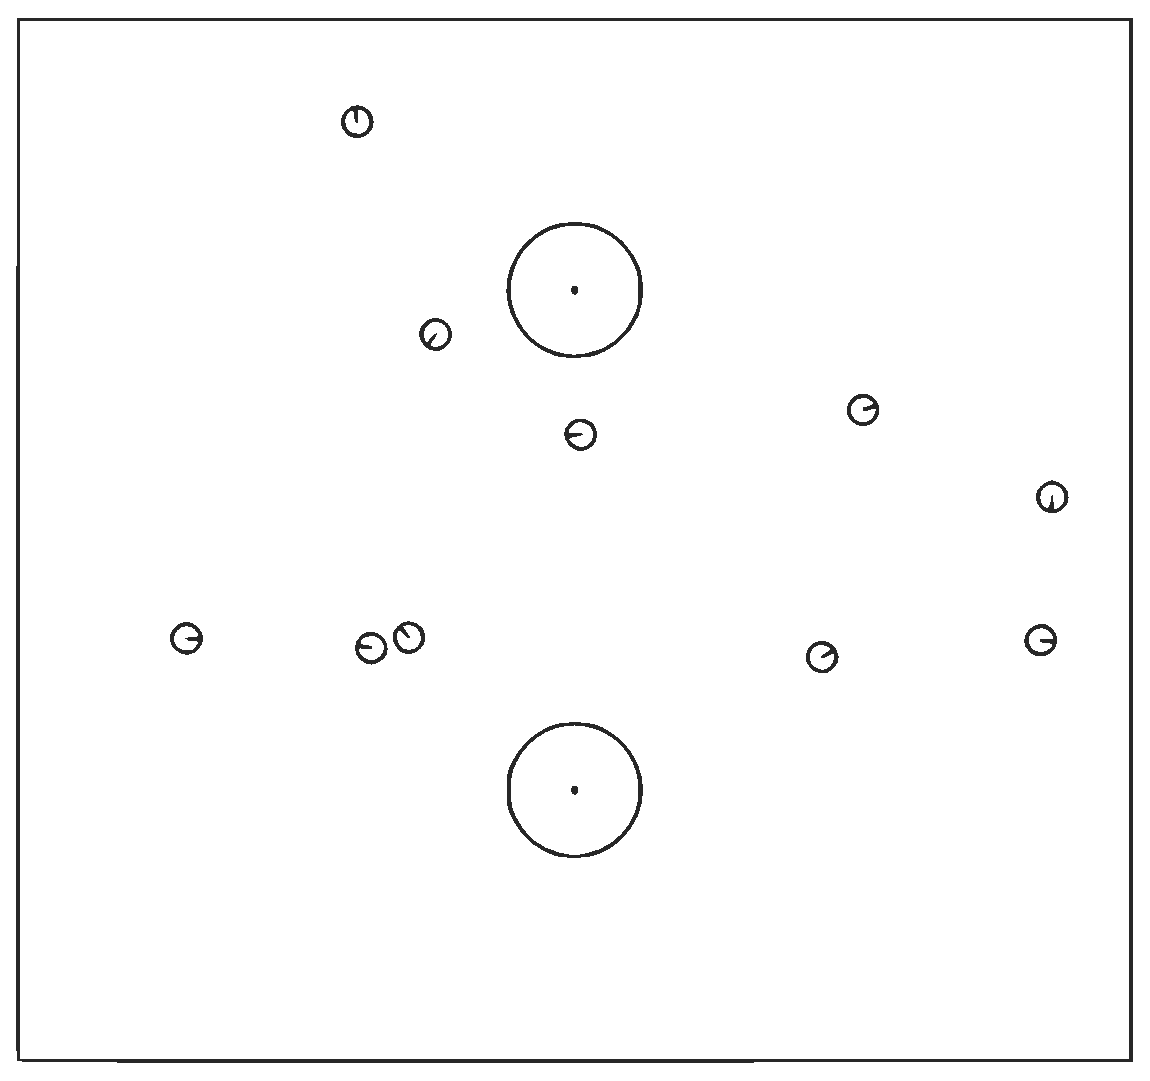
\includegraphics[width=\textwidth]{figures/simulation-28-t0-bold}
        \subcaption{T = 0 s}
    \end{minipage}%
    \begin{minipage}{.3\textwidth}
        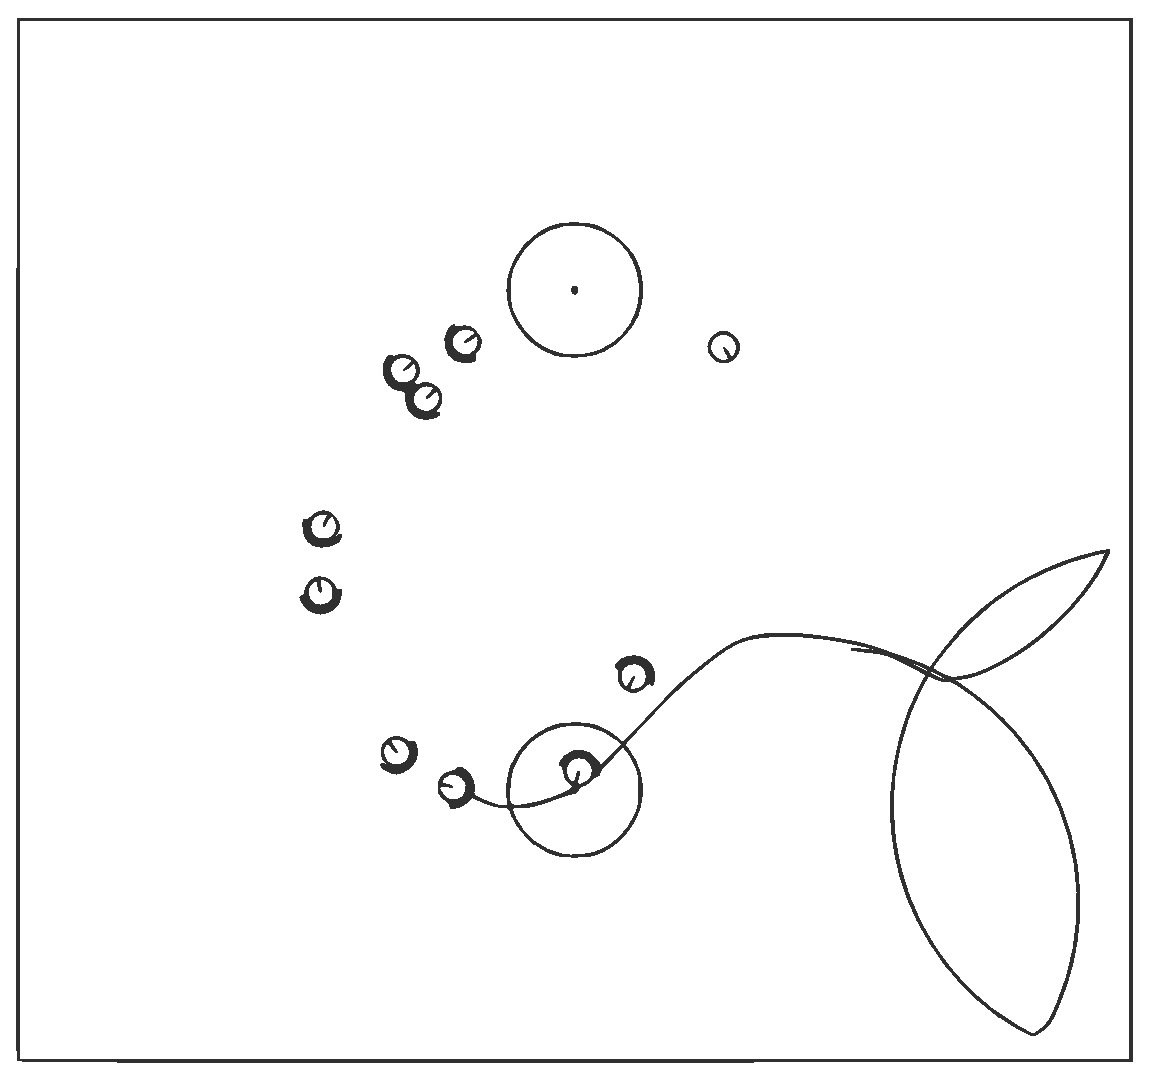
\includegraphics[width=\textwidth]{figures/simulation-28-t60-bold}
        \subcaption{T = 60 s}
    \end{minipage}%
    \begin{minipage}{.3\textwidth}
        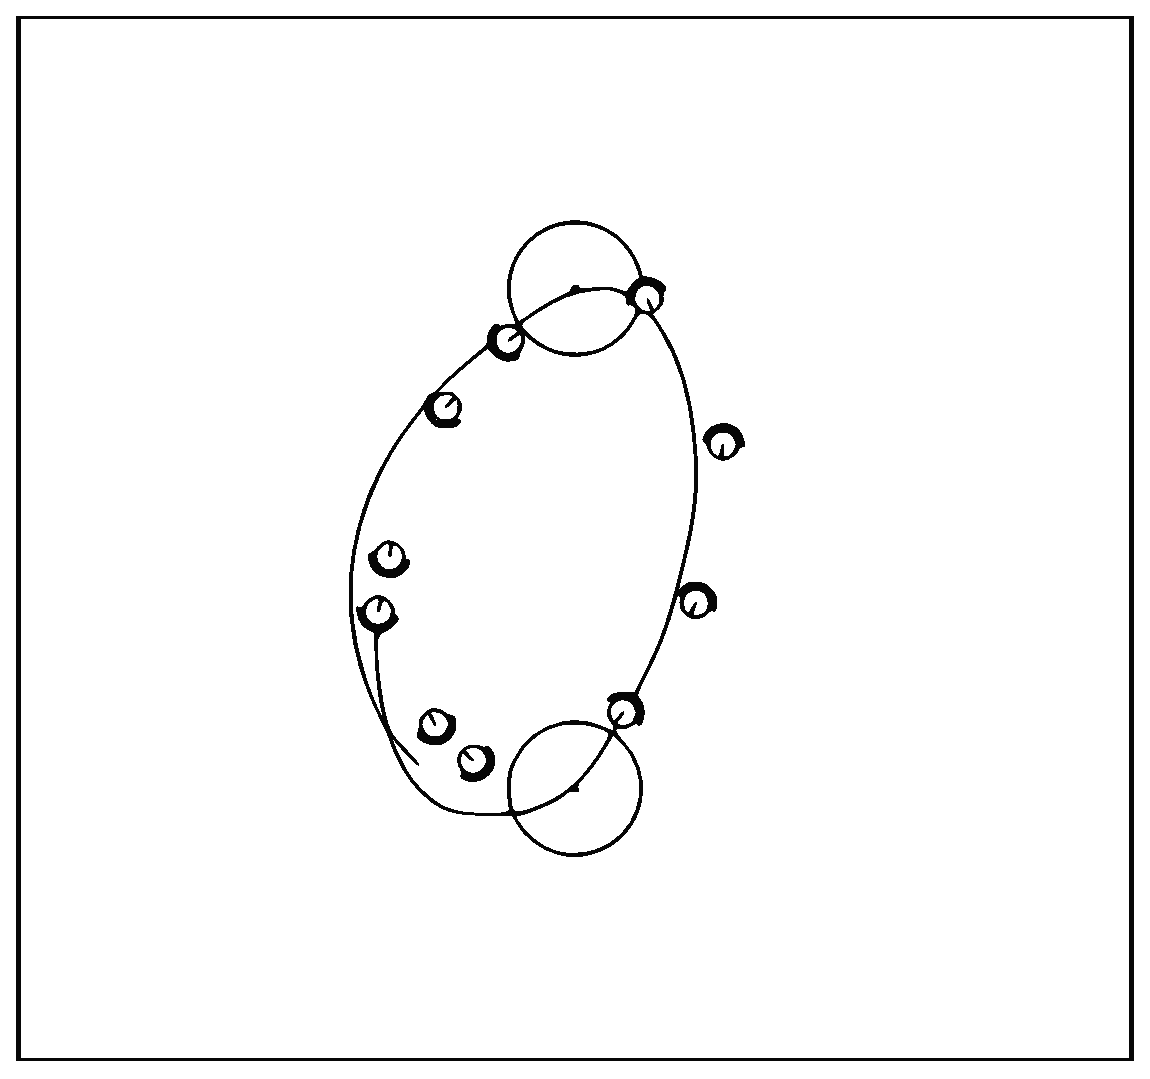
\includegraphics[width=\textwidth]{figures/simulation-28-t120-bold}
        \subcaption{T = 120 s}
    \end{minipage}

    \caption{Simulação a partir da solução resultante de uma execução típica do GA}
    \label{fig:sim}
\end{figure}

No início da simulação ocorre uma fase de exploração do ambiente em busca das áreas alvo. No momento em que um dos robôs encontra uma área alvo, ele liga o LED traseiro. Outros robôs suficientemente próximos a ele conseguem detectar esse sinal e, por consequência passam a segui-lo e também ligam seus LEDs traseiros. Assim sucessivamente até que todos os robôs formem uma cadeia, ou seja, um caminho entre as áreas alvo.

A partir de observações preliminares, nota-se que em simulações cuja função de \fitness F resulta em valores menores do que $0,10$ não há comportamento coletivo e o objetivo não é alcançado. Nos outros casos, quanto maior o resultado da função F, menor é o tamanho do caminho desempenhado por cada robô para deslocar-se de uma área alvo à outra.

\section{Comparações entre funções de \fitness}

A Figura \ref{fig:func-fitness-gen} mostra a evolução das populações (\fitness média e máxima) durante a execução de um GA para cada função de \fitness diferente. O melhor desempenho é apresentado pela função \textbf{f3} e o pior pela função \textbf{f1}.

\begin{figure}[h]
    \centering
    \begin{minipage}{.5\textwidth}
        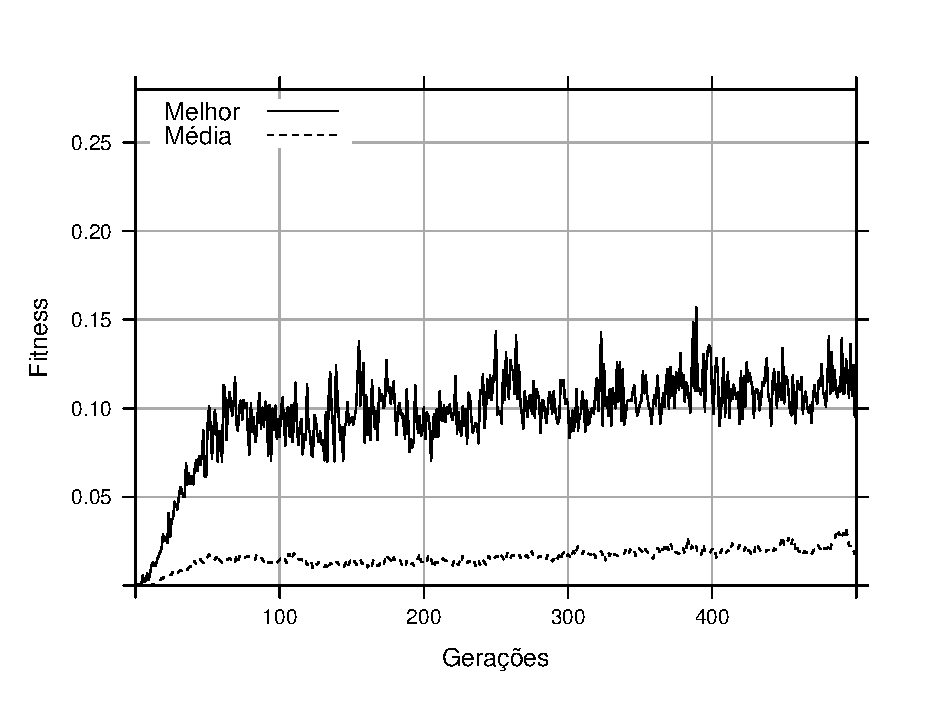
\includegraphics[width=\textwidth]{figures/fitness-f1}
        \subcaption{Função de \fitness \textbf{f1}}
    \end{minipage}%
    \begin{minipage}{.5\textwidth}
        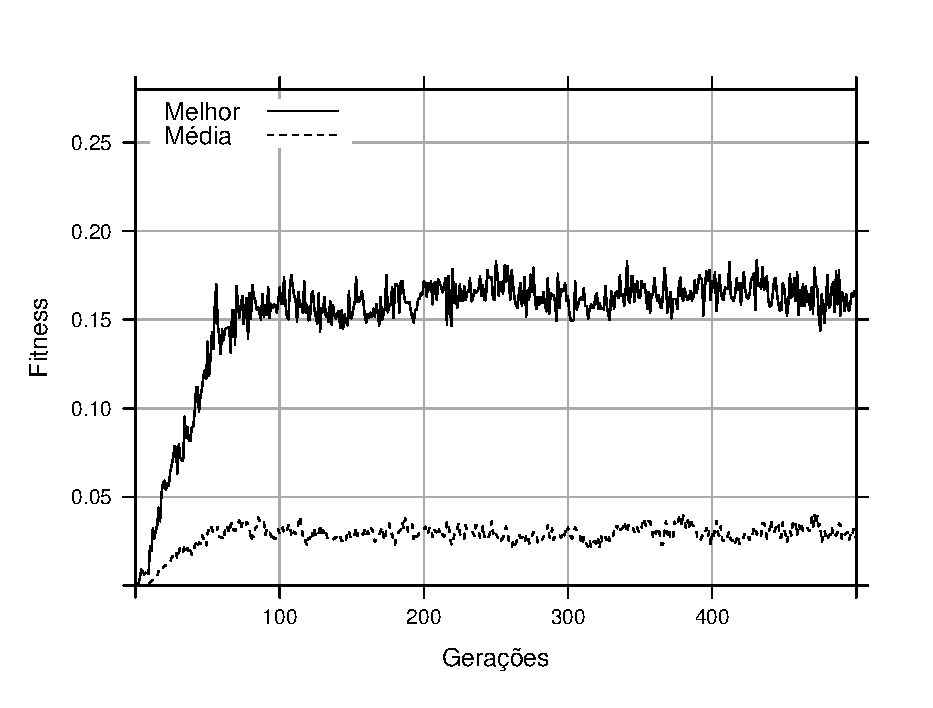
\includegraphics[width=\textwidth]{figures/fitness-f2}
        \subcaption{Função de \fitness \textbf{f2}}
    \end{minipage}

    \begin{minipage}{.5\textwidth}
        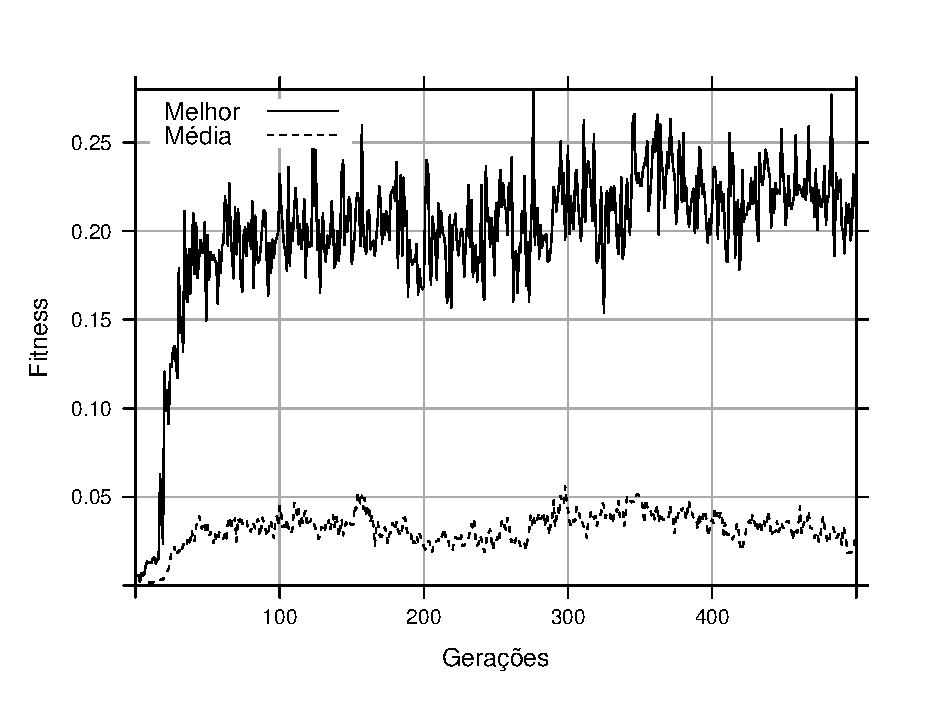
\includegraphics[width=\textwidth]{figures/fitness-f3}
        \subcaption{Função de \fitness \textbf{f3}}
    \end{minipage}%
    \begin{minipage}{.5\textwidth}
        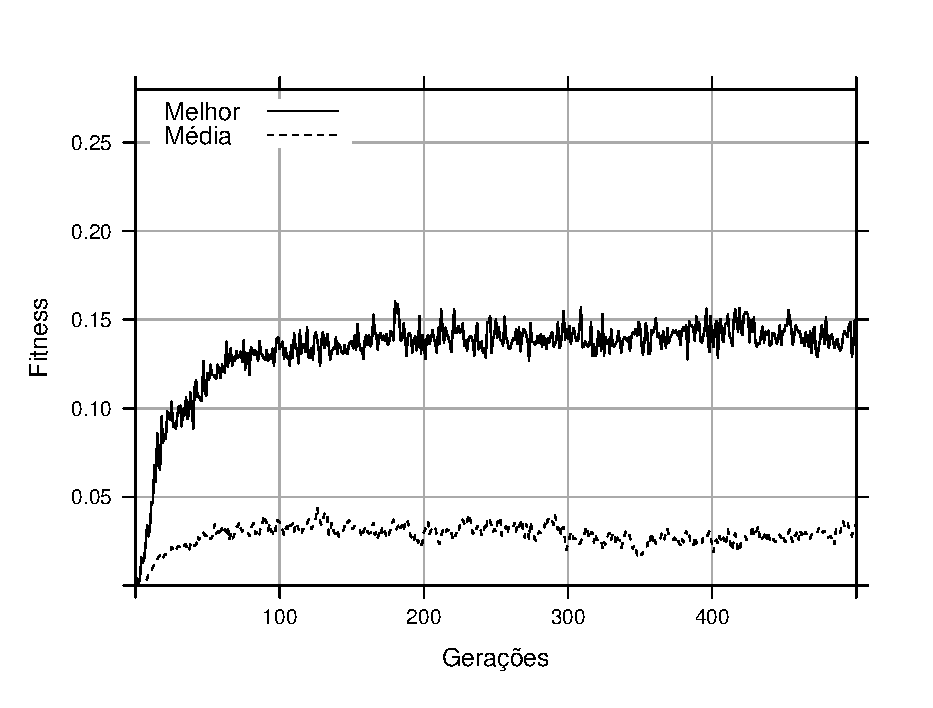
\includegraphics[width=\textwidth]{figures/fitness-f4}
        \subcaption{Função de \fitness \textbf{f4}}
    \end{minipage}

    \caption{Gráfico da \fitness do melhor indivíduo e média das \fitnessp dos indivíduos da população ao longo das gerações da execução de um GA para cada uma das quatro funções de \fitness.}
    \label{fig:func-fitness-gen}
\end{figure}

O melhor indivíduo resultante do algoritmo de treinamento com alguma das funções de \fitness deve ser apto a reproduzir o mesmo comportamento no ambiente real onde a posição das áreas alvo é totalmente aleatória. A função de \fitness F contempla esse ambiente real. Por isso, utilizaremos a função F para estimar o desempenho de um indivíduo (após treinamento) em uma situação real.

A Figura \ref{fig:reeval} informa o resultado de 500 avaliações da função de \fitness F a partir das soluções resultantes da execução de um GA para cada função de \fitness (ambientes de treinamento).

Contraditoriamente, o desempenho da função \textbf{f3} é o pior dentre os quatro nessas condições.

\begin{figure}[h]
    \centering
    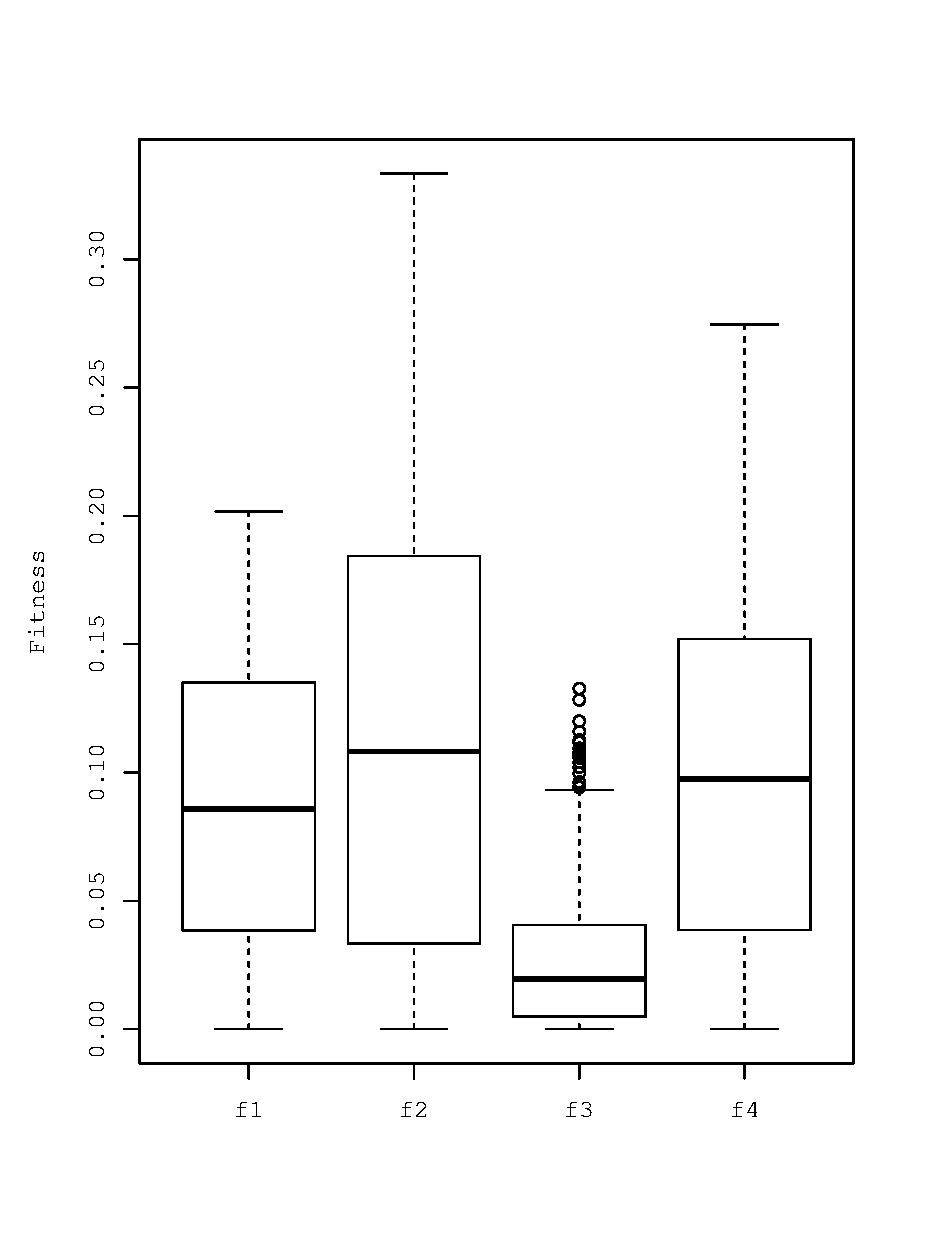
\includegraphics[width=.4\textwidth]{figures/reeval}
    \caption{Gráfico \textit{boxplot} com o resultado de 500 avaliações da função de \fitness F a partir das soluções resultantes da execução de um GA para cada função de \fitness.}
    \label{fig:reeval}
\end{figure}

A solução resultante da execução com a função \textbf{f3} explora o fato de que a distância entre as áreas alvo é sempre a mesma para todos os testes, daí o baixo desempenho quando reavaliada no contexto da situação real na qual a distância varia aleatoriamente.

As funções \textbf{f2} e \textbf{f4} de fato levam a melhores soluções do que a função \textbf{f1}. Como discutido na Seção \ref{sec:exp-fitness}, a aleatoriedade, mais presente na função \textbf{f1}, atrapalha a evolução.

%%%%%%%%%%%%%%%%%%%%%%%%%%%%%%%%%%%%%%%%%%%%%%%%%%%%%%%%%%%%%%%%%%%%%%%%%%%%%%%%%%%%%%%%%%%%%%%%%%%

\pagebreak

\section{Comparações entre algoritmos de treinamento}

\begin{figure}[H]
    \centering
    \begin{minipage}{.47\textwidth}
        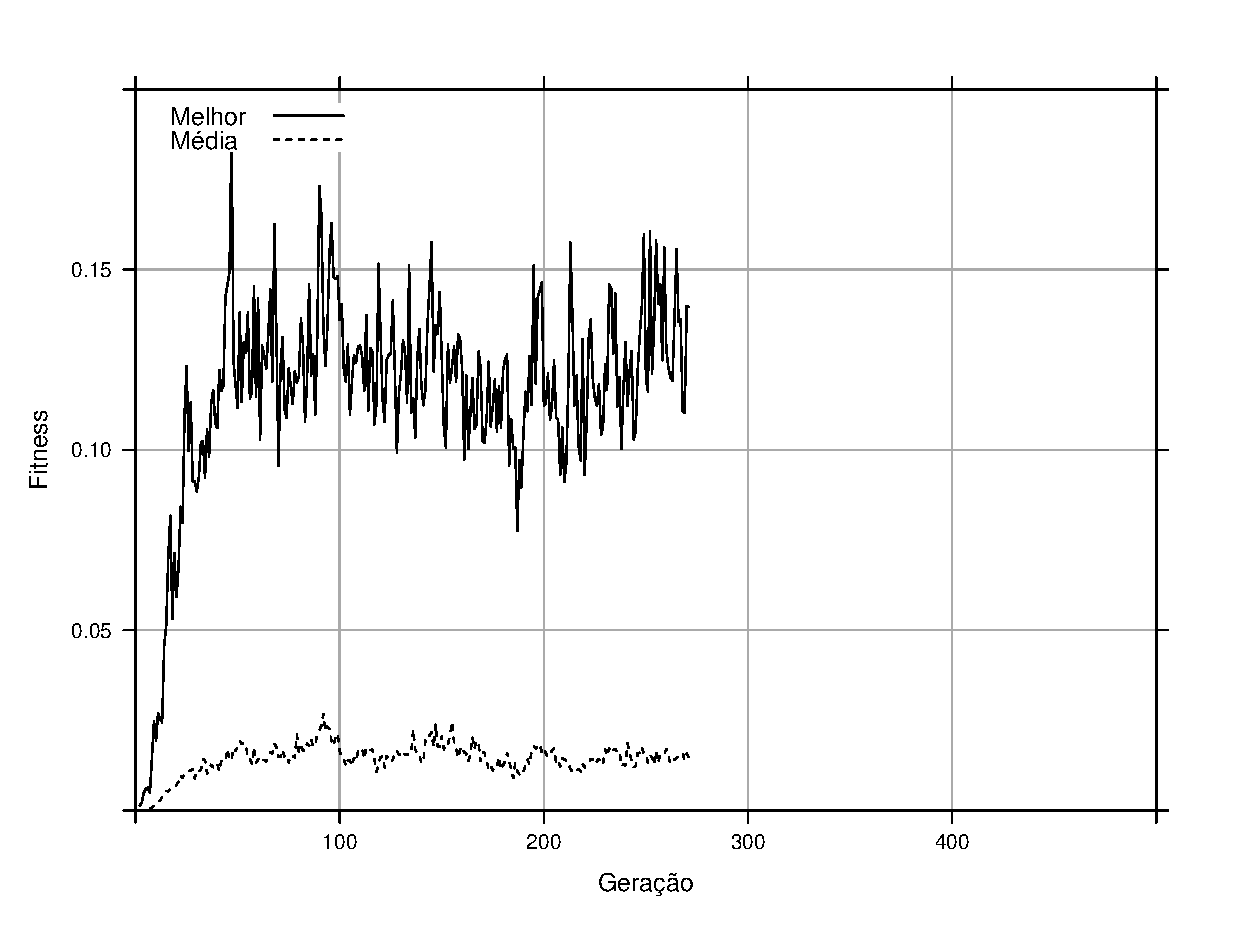
\includegraphics[width=\textwidth]{figures/fitness-GA}
        \subcaption{Execução de um GA}
    \end{minipage}%
    \begin{minipage}{.47\textwidth}
        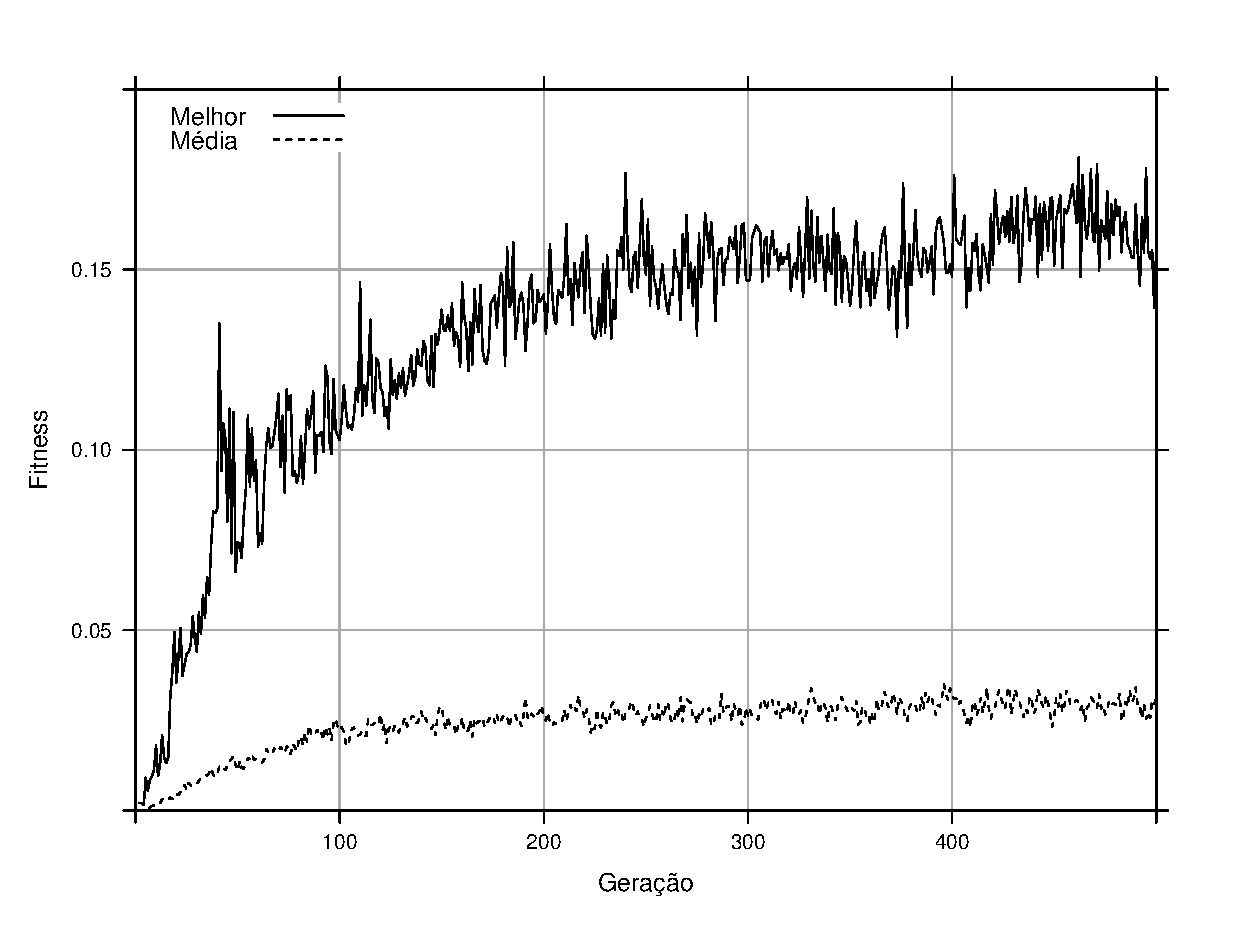
\includegraphics[width=\textwidth]{figures/fitness-PGA}
        \subcaption{Execução de um CGPGA}
    \end{minipage}

    \begin{minipage}{.47\textwidth}
        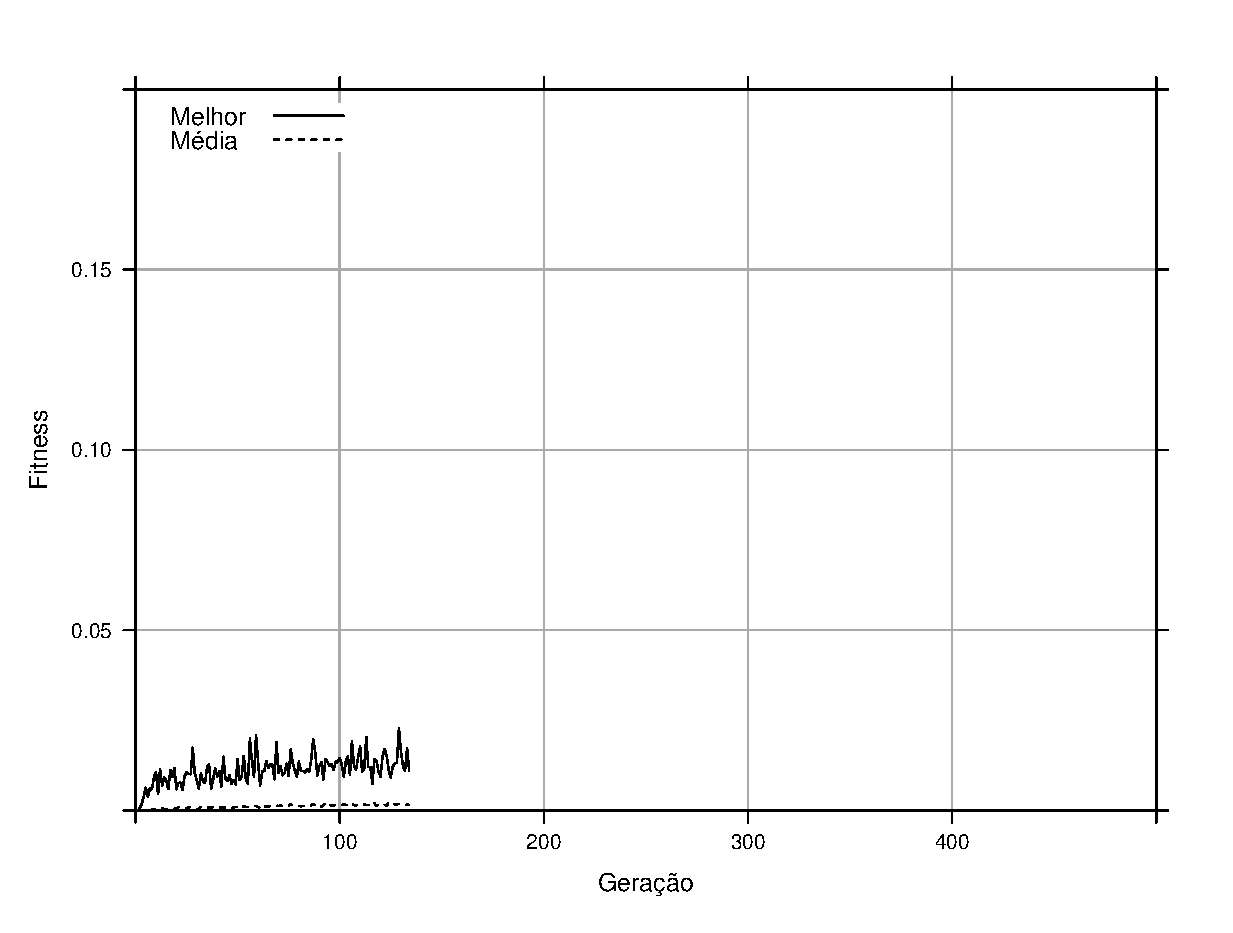
\includegraphics[width=\textwidth]{figures/fitness-PSO}
        \subcaption{Execução de um PSO}
    \end{minipage}%
    \begin{minipage}{.47\textwidth}
        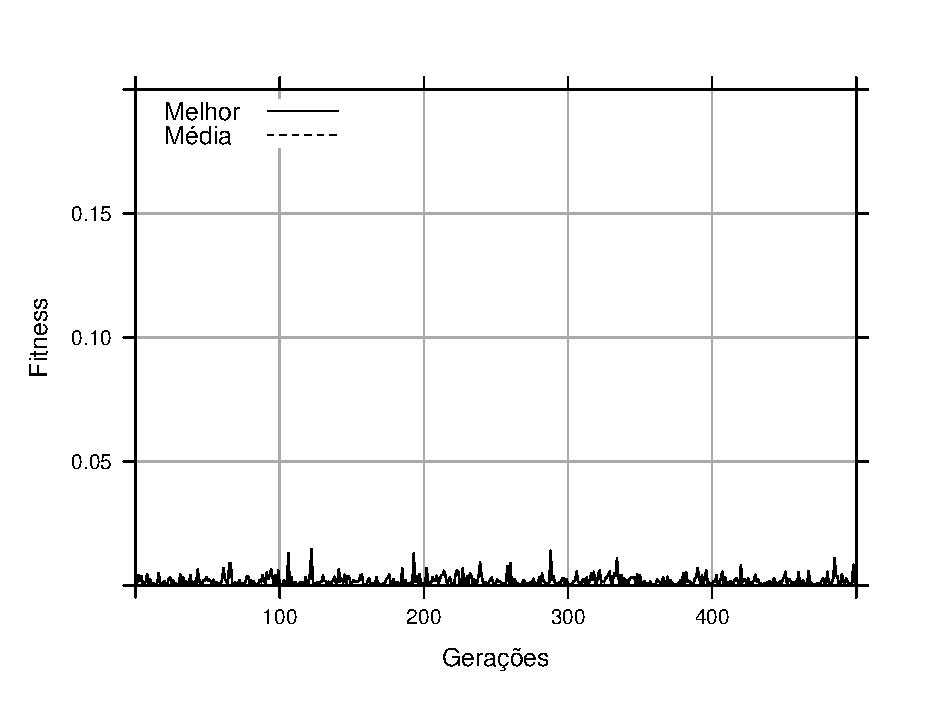
\includegraphics[width=\textwidth]{figures/fitness-DPSO}
        \subcaption{Execução de um DPSO}
    \end{minipage}

    \caption{Gráfico da \fitness do melhor indivíduo e média das \fitnessp dos indivíduos da população ao longo das gerações de uma execução típica para cada um dos quatro algoritmos.}
    \label{fig:fitness-gen}
\end{figure}

\begin{figure}[H]
    \centering
    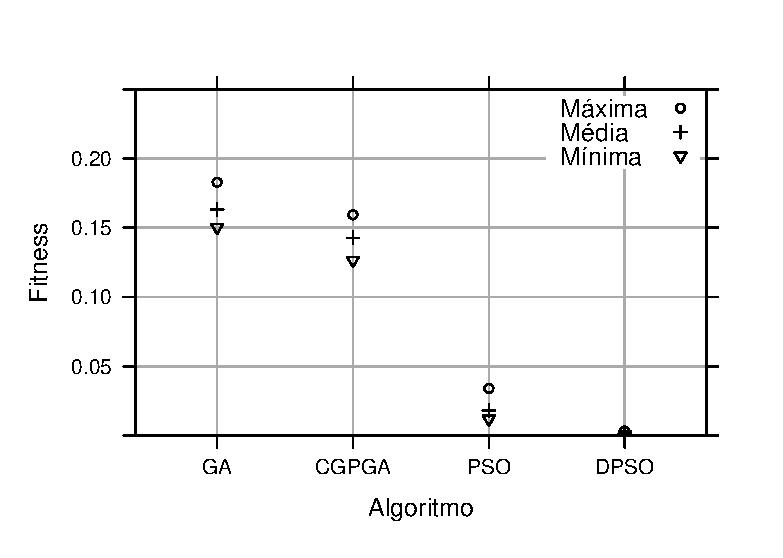
\includegraphics[width=.5\textwidth]{figures/compare}
    \caption{Gráfico da \fitness resultante máxima, média e mínima entre 5 execuções para cada um dos algoritmos.}
    \label{fig:compare}
\end{figure}

\pagebreak

A Figura \ref{fig:fitness-gen} apresenta a evolução das população ao longo das gerações em uma execução típica para os quatro algoritmos de treinamento selecionados.

A Figura \ref{fig:compare} informa a \fitness resultante máxima, média e mínima entre 5 execuções para cada um dos algoritmos. Observe que a \fitness resultante provém do melhor indivíduo na última geração.

O CGPGA não apresenta melhoras em relação ao GA. Para este problema, a divisão das populações em ilhas não favorece de maneira alguma a exploração do espaço de busca.

O desempenho do PSO é baixo porque provavelmente as partículas convergem muito rapidamente para um máximo local, assim perdendo diversidade. Acredita-se mutação do GA é o fator que impede tal convergência prematura.

No DPSO, o espaço de busca é maior porque, como visto na Seção \ref{sub:dpso}, o que está sendo otimizado pelo algoritmo não é a solução em si, mas sim a probabilidade da solução assumir determinado valor. Acredita-se que isso é o fator que leva ao desempenho baixo desse algoritmo para esse problema.

\subsection{Ajuste de parâmetros}

Os parâmetros do GA (e consequentemente do CGPGA) foram inicialmente escolhidos com base nos experimentos realizados por Sperati et al. \cite{sperati2011path}. Em experimentos preliminares, notou-se baixa correlação entre a qualidade da solução e a taxa de cruzamento. Todavia, a estategia é sen o elitismo e a taxa de mutação são bastante sensíveis como pode ser visto na Figura \ref{fig:mut-elite}.

\begin{figure}[H]
    \centering
    \begin{minipage}{.47\textwidth}
        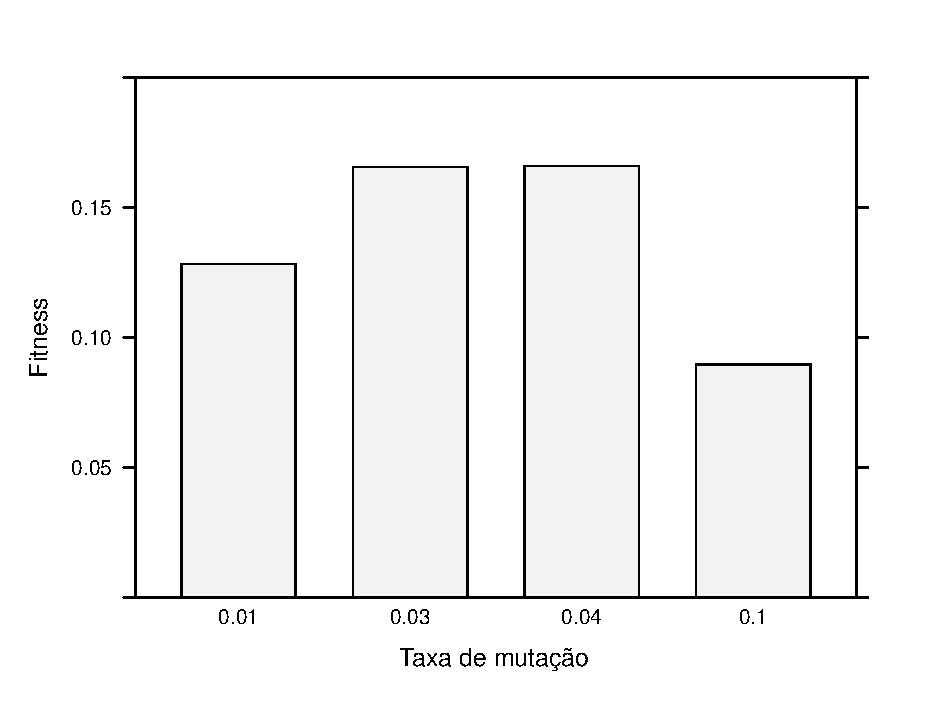
\includegraphics[width=\textwidth]{figures/mutation}
    \end{minipage}%
    \quad\quad\quad\quad
    \begin{minipage}{.35\textwidth}
        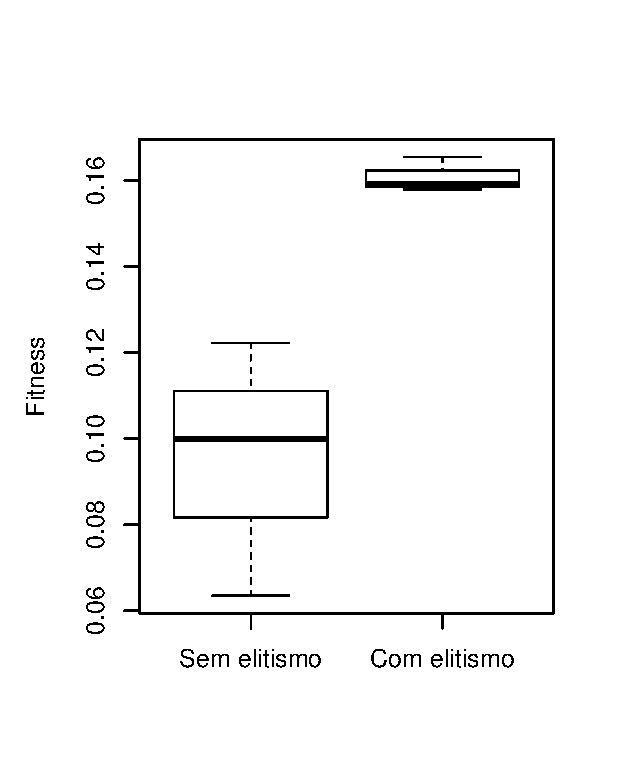
\includegraphics[width=\textwidth]{figures/elitism}
    \end{minipage}

    \caption{Gráficos de linhas da \fitness resultante na execução de um GA para cada taxa de mutação escolhida e gráfico \textit{boxplot} da \fitness em 3 execuções com elitismo e 3 execuções sem elitismo}
    \label{fig:mut-elite}
\end{figure}

Observou-se que a mutação é crucial para que o algoritmo não fique preso em máximos locais, mas em exagero ocasiona muita perturbação e impede a evolução da população. O elitismo impede que boas soluções sejam perdidas facilmente ao longo da evolução.